\documentclass{article}
\usepackage{times}
\usepackage{graphicx}
\usepackage{subfigure} 
\usepackage{natbib}
\usepackage{algorithm}
\usepackage{amsmath}
\usepackage{amsfonts}
\usepackage{algorithmic}
\usepackage{subfigure}
\usepackage{hyperref}
\newcommand{\theHalgorithm}{\arabic{algorithm}} % Fixes misbehavior of conflicting packages.
\usepackage{icml2016/icml2016} 
\usepackage[nolist]{acronym} % Acronym package -- give argument <dua> to suppress acronym usage


\icmltitlerunning{Approximate State Abstraction}

% --- Notation Commands ---
\newcommand{\ep}{\widetilde \phi}
\newcommand{\epQ}{\ep_{Q^*}}
\newcommand\defn[1]{{\bf Definition:} #1}
\DeclareMathOperator*{\argmin}{arg\,min}
\DeclareMathOperator*{\argmax}{arg\,max}


% --- Note Commands ---
\usepackage{color}
\newcommand\dnote[1]{\textcolor{blue}{Dave: #1}}
\newcommand\enote[1]{\textcolor{green}{Ellis: #1}}

% --- DOCUMENT ---
\begin{document}

\twocolumn[
\icmltitle{Approximate State Abstraction}

% Paper Meta Info
\icmlauthor{David Abel}{david_abel@brown.edu}
\icmladdress{Brown University,
            115 Waterman Street, Providence, RI 02906}
\icmlauthor{D. Ellis Hershkowitz}{david_hershkowitz@brown.edu}
\icmladdress{Brown University,
            115 Waterman Street, Providence, RI 02906}
\icmlauthor{Michael L.\ Littman}{michael_littman@brown.edu}
\icmladdress{Brown University,
            115 Waterman Street, Providence, RI 02906}
    
\icmlkeywords{Reinforcement Learning, State Aggregation, State Abstraction, Planning, MDP}
            
\vskip 0.3in
]


%Acronyms -- use \ac for acronym or \acp for plural/capitalization of acronym
\begin{acronym}
\acro{MDP}{Markov Decision Process}
\acrodefplural{MDP}[MDPs]{Markov Decision Processes}
\acro{RL}{reinforcement learning}
\acrodefplural{RL}{Reinforcement learning}
\end{acronym}


% --- ABSTRACT ---
\begin{abstract}
The combinatorial explosion that plagues planning and \ac{RL} algorithms can be overcome using abstraction. For instance, prohibitively difficult task representations can be condensed, preserving essential information such that solutions are tractably computable. In this work, we investigate a theoretical framework for approximate state abstraction that achieves high degrees of compressing while preserving near optimal behavior. \acp{RL} agents using these abstractions treat experiences that resemble each other as equivalent, and generalize knowledge to novel scenarios based on prior experiences. We present theoretical guarantees of the quality of value functions derived from four classes of approximate state abstraction. Additionally, we empirically evaluate the relationship between the degree of approximation and the degree of abstraction achieved in a variety of tasks, as well as the tradeoff between approximation magnitude and optimality of behavior.
\end{abstract}


% --- SECTION: Introduction ---
\section{Introduction}
Abstraction plays a fundamental role in learning. Through abstraction, intelligent agents may reason about only the salient features of their environment while ignoring what is irrelevant, consequently enabling agents to solve considerably more complex problems. However, the knowledge available to a learning agent at any given moment is approximate \dnote{Change this sentence}. Thus, agents must determine when their knowledge is sufficiently accurate to form the basis of abstraction. This work characterizes what is ``sufficiently accurate" information for abstraction amounts to in the context of planning and \ac{RL} in \acp{MDP}.

% Abstraction is a good idea b/c MDP has poly comp comp and samp comp in S, but S grows fast.
Solving for optimal behavior in \acp{MDP} in a planning setting is known to be P-Complete in the size of the state space~\cite{littman1995complexity,papadimitriou1987complexity}. Similarly, many \ac{RL} algorithms for solving \acp{MDP} are known to require a number of samples polynomial in the size of the state space~\cite{strehl2009reinforcement}. Although polynomial runtime or sample complexity may seem like a reasonable constraint, due to Bellman's curse of dimensionality the size of the state space of an \ac{MDP} grows super-polynomially with the number of variables that characterize the domain. Thus, polynomial behavior in state space size often translates to intractability for sufficiently complicated tasks. \dnote{Would prefer a different example} For instance, a robot involved in a pick and place task might be able employ planning algorithms to solve for how to manipulate some objects into a desired configuration in time polynomial in the number of states, but the number of states it must consider to do so grows exponentially with the number of objects it plans over CITE DABE ICAPS.

% Existing work on state abstraction.
Thus, a key research agenda for planning and RL is leveraging abstraction in order to reduce large state spaces~\cite{andre2002state,jong2005state,dietterich2000hierarchical,Bean2011}. These methods are characterized by reducing \textit{ground} MDPs with large state spaces to \textit{abstract} MDPs with smaller state spaces by aggregating states according to some notion of equality or similarity. Existing work has characterized how aggregation of states with equal values of particular quantities fully maintain optimality~\cite{li2006towards,dean1997modelmin}. However, exactly solving for these quantities is itself computationally taxing and often as difficult as solving for optimal behavior in the ground \ac{MDP}, thereby defeating the purpose of abstraction.

% Approximate abstraction
In this work we demonstrate that aggregation of states on the basis of various approximate criteria incur only bounded error in the resulting policy. Relaxing the aggregation criteria from equality of quantities to $\varepsilon$-closeness offers two benefits. First, state aggregation algorithms that satisfy these criteria employ the sort of knowledge which we expect a planning or learning algorithm to approximate without fully solving the \ac{MDP}. Second, because the state aggregation criteria are relaxed to approximate equality, methods which employ approximate equality are able to tune the aggressiveness of state aggregation all the while incurring bounded error.

% Summary	
This paper is organized as follows. We first introduce the necessary terminology and background of \ac{RL} and state abstraction. We then survey existing approaches in state abstraction as applied to sequential decision making. The following section introduces our four primary results; bounds on the error guaranteed by four classes of approximate state abstraction. We then discuss our experimentation, in which we apply one class of approximate abstraction to a variety of different tasks, visualizing their abstraction and showing the relationship between degrees of compression and error incurred.


% --- SECTION: Background ---
\section{Background}

%MDP/SDM Background and Notation
\subsection{\acp{MDP} and Sequential Decision Making}
A \ac{MDP} is a five-tuple: $\langle \mathcal{S}, \mathcal{A}, \mathcal{T}, \mathcal{R}, \gamma \rangle$: $\mathcal{S}$ is a finite state space; $\mathcal{A}$ is the set of actions available to the agent; $\mathcal{T}$ denotes $\mathcal{T}(s' \mid s,a)$, the probability of an agent applying action $a \in \mathcal{A}$ in state $s \in \mathcal{S}$ and arriving in $s' \in \mathcal{S}$; $\mathcal{R}(s)$ denotes the reward received by the agent arriving in state $s$; $\gamma \in [0, 1]$ is a discount  factor that defines how much the agent prefers immediate rewards over future rewards. We assume without loss of generality that all reward functions are normalized to $[0,1]$.

The goal of an agent in an \ac{MDP} is to solve for a policy that maps states to actions: $\pi: \mathcal{S} \rightarrow \mathcal{A}$. In particular, the agent wants to solve for the policy that maximizes its expected discounted reward from any state. This goal policy is denoted $\pi^*$. We denote the expected discounted reward for following policy $\pi$ from state $s$ as the value of the state under that policy, $V(s)^\pi$. We similarly denote the expected discounted reward for taking action $a \in \mathcal{A}$ and then following policy $\pi$ from state $s$ forever after as $Q^\pi(s,a)$. Lastly, we denote the value and $Q$ functions under the optimal policy as $V^*$ and $Q^*$ respectively. \enote{Add citation -- either Littman review paper or Sutton/Barto}

\enote{Define value of state under a policy}

%Lihong Section
\subsection{Abstraction Notation}
We build upon the notation used by \cite{li2006towards} \enote{This should probably say more}.

We understand an abstraction as a mapping from a ground MDP $M_G$ to an abstract MDP $M_A$ using a state aggregation scheme. $M_G = \langle \mathcal{S}_G, \mathcal{A}, \mathcal{T}_G, \mathcal{R}_G, \gamma \rangle$ and $M_A = \langle \mathcal{S}_A, \mathcal{A}, \mathcal{T}_A, \mathcal{R}_A, \gamma \rangle$.

% States
The states in the abstract MDP are constructed by applying a state aggregation scheme, $\phi$, to the states in the ground MDP, $\mathcal{S}_A$. More specifically, $\phi$ maps a state in the ground MDP to a state in the abstract MDP.
\begin{equation}
\mathcal{S}_A = \{ \phi(s) \mid s \in \mathcal{S}_G\}
\end{equation}

Intuitively, the abstract reward function and abstract transition dynamics for each abstract state are a weighted combination of the rewards and transitions for each ground state in the partition. We make no assumptions about the weighting scheme, except that the weighting is a convex combination across all states in the partition.

% Reward
The abstract reward function $\mathcal{R}_A(s,a)$ is a weighted sum of the rewards of each of the ground states that map to the abstract state:
\begin{equation}
\mathcal{R}_A(s,a) = \sum_{g \in \phi(s), s \in \mathcal{S}_G} \mathcal{R}_G(g,a) \omega(g) 
\end{equation}


% Transition
The abstract transition function $\mathcal{T}_A(s,a,s')$ is a weighted sum of the transitions of each of the ground states that map to the abstract state:
\begin{equation}
\mathcal{T}_A(s,a,s') = \sum_{g \in \phi^{-1}(s)} \sum_{g' \in \phi^{-1}(s')} \mathcal{T}_G(g,a,g') \omega(g) 
\end{equation}
For:
\begin{equation}
s, s' \in \mathcal{S}_A
\end{equation}

% Abstract policy using in ground.
In general we are interested in how policies defined over the abstract MDP perform in the ground MDP. To leverage a policy defined in the abstract in the ground, we map a ground state into the abstract state space, and query the abstract policy for behavior. Specifically:
\begin{equation}
\pi_A(s) = \pi_A(\phi(s)),\ s \in \mathcal{S}_G
\end{equation}

We evaluate the value of the abstract policy in the ground MDP by following the abstract policy:
\begin{equation}
V^{\pi_A}(s) = \mathcal{R}_G(s,\pi_A(a)) + \gamma \sum_{s' \in \mathcal{S}_G} \mathcal{T}_G(s,\pi_A(a),s')V^{\pi_A}(s')
\end{equation}

\enote{Define $V_G$ and $V_A$ (value function in ground and value function in abstract)}

% Subsection: Exact Abstraction Framework
\subsection{Exact Abstraction Framework}

\citep{li2006towards} develop a framework for state abstraction in \acp{MDP}, the notation for which is defined in the previous section. Here we survey their main results that we extend to the framework of approximate abstraction.

In particular, they define the following five classes of state abstractors, inspired by existing methods for state abstraction in \acp{MDP}. For brevity, we include those which we build upon directly (see their paper for full details).

\defn{A $Q^*$-irrelevance abstraction, $\phi_{Q^*}$, is such that:
\begin{equation}
\phi_{Q^*}(s_1) = \phi_{Q^*}(s_2) \longrightarrow \forall a\ \left(Q^*(s_1,a) = Q^*(s_2,a)\right)
\end{equation}
}

\defn{A model-irrelevance abstraction, $\phi_{model}$, is such that:
\begin{multline}
\phi_{model}(s_1) = \phi_{model}(s_2) \rightarrow \forall a\ \mathcal{R}_G(s_1,a) = \mathcal{R}_G(s_2,a) \\
\end{multline}
And:
\begin{multline}
\phi_{model}(s_1) = \phi_{model}(s_2) \rightarrow \\ \forall a \sum_{s' \in \phi^{-1}(\phi(s_1))} \mathcal{T}_G(s_1,a,s') =\sum_{s' \in \phi^{-1}(\phi(s_2))} \mathcal{T}_G(s_2,a,s') \\
\end{multline}
}


% --- SECTION: Related Work ---
\section{Related Work}


% Approximate abstraction work.
%Dean: 
%\begin{itemize}
%\item \citep{dean1997model} Does abstraction with model equality.
%\item \citep{dean1997modelmin} Does approximate abstraction with model similarity.
%\end{itemize}
%
%Boutilier:
%\begin{itemize}
%\item ~\citep{dearden1997abstraction} Abstraction: a similar ish bound with a similar is agenda.
%\item ~\citep{Boutilier2000} Stochastic DP: tree based policies, sort of bound thingies.
%\end{itemize}
%
%Even~\cite{even2003approximate}: COLT paper on different metrics
%
%Ortner:
%\begin{itemize}
%\item ~\cite{ortner2013adaptive}: Uses Dean results to do UCRL online learning of abstraction. 
%\item ~\cite{odalric2013optimal}: Learn which abstraction to use online (similar to the Nan paper)
%\end{itemize}


\subsection{Approximate State Abstraction}
\citep{dean1997model} investigates partitioning an MDP's state space into $\epsilon$-homogenous blocks, which are defined as clusters of states whose transition model and reward function are within $\epsilon$ of each other. They provide bounds on the error incurred as a result of using the optimal policy defined over these blocks in the original MDP. This method of abstraction is effectively characterized as a function belonging to the approximate class $\phi_{model}$.
Several approaches build on the notion of $\epsilon$-homogeneity. ~\citep{even2003approximate} analyze different distant metrics used in the process of identifying $\epsilon$-homogenous partitions. ~\cite{ortner2013adaptive} develops an algorithm for learning partitions in an on line setting by taking advantage of the confidence bounds for $T$ and $R$ provided by UCRL~\cite{auer2009near}.

%Prior work considers abstractions related to transition model similarity, or both transition model and reward function similarity with the aim of reducing the state space size required for planning and learning while still achieving a bounded error solution~\cite{even2003approximate,ortner2013adaptive,Boutilier2000}. All of this work is closely in line with our own agenda; they investigate rules for abstractions that may inform a reduced, abstract MDP, the solution to which has bounded error in the original MDP. However, all prior results explore model similarity abstraction rules, whereas we consider several broader classes of approximate abstraction. Furthermore, our results depend on no assumptions regarding the structure of the MDPs in which we apply our abstraction, and generalize to both the reinforcement learning or the planning setting, while many previous approaches require simplifying assumptions about the space of MDPs\dnote{a comment about what assumptions are made would be nice}, or only work target planning.

\subsection{Specific Abstraction Algorithms}
Many previous works have targeted the creation of algorithms that enable state abstraction for MDPs. \citep{andre2002state} investigates a method for state abstraction in hierarchical reinforcement learning leveraging a programming language called ALISP that promotes the notion of {\it safe} state abstraction. Agents programmed using ALISP can ignore irrelevant parts of the state, achieving abstraction that maintains optimality. ~\cite{dietterich2000hierarchical} develops the MAXQ algorithm, a framework for composing tasks into an abstracted hierarchy. \citep{jong2005state} introduce a method called {\it policy-irrelevance}, in which agents identify (online) which state variables may be safely ignored in a factored MDP, and consequently achieve state abstraction. The agent will learn to ignore state variables that don't impact optimal behavior, and is consequently contained within the approximate $\phi_{a^*}$ work. For a full survey of algorithms that leverage state abstraction in recent reinforcement learning literature, see~\cite{li2006towards}.


% Other? Selecting abstractions
%\subsection{Selecting Abstractions}
%\citep{jiang2015abstraction} investigate the question of choosing between two abstractions during learning. They provide analysis for an online approach to identifying the better abstraction. 

% Defining 

% Critically, our work differs from these in that our primary aim is to achieve understanding of what methods of abstraction in reinforcement learning can maintain bounded error solutions, while these focus on particular strategies that fit within our framework.

% Lihong/Walsh/Littman: Towards a unified theory...

%\begin{itemize}
%\item {\bf Approximate equivalence of MDP}~\cite{even2003approximate}
%\item ALisp~\cite{andre2002state}
%\item Aggregation in DP~\cite{Bean2011}
%\item {\bf Does approximate aggregation and then UCRL}~\cite{ortner2013adaptive}
%Very similar to our overall goal: learn an abstraction function online using confidence bounds as the epsilon. Wowza. Only uses the whole model similarity business though. Seems to be the case for all of the approximate aggregation work (just does the bisimulation or $\epsilon-homogeneity$)
%
%\item Selecting the state rep in RL~\cite{maillard2011selecting}
%\item Near optimal state reps~\cite{ortner2014selecting}
%\item SMDP homomorphisms~\cite{ravindran2003smdp}
%\end{itemize}


% --- SECTION: State Abstraction ---
\section{Approximate State Abstraction}

% Intro to approx state abstraction results.
Here we introduce our formal method for approximate state abstraction, and the related results bounding the error associated with these abstraction methods. In particular, we demonstrate that abstractions based on $Q^*$ similarity, Model similarity (that is, $\mathcal{T}$ and $\mathcal{R}$), and similarity between distributions over $Q^*$, for both multinomial and Boltzmann disibtruions, induce abstract MDPs for which the optimal policy has bounded error in the ground MDP.

In general, our proof strategy for each of the included results is as follows:
\begin{itemize}
\item First, we relate the values of states in the ground MDP to value of the states in the Abstract MDP
\item Then, we relate the value of states in the ground MDP to value of the states in the Abstract MDP under the optimal abstract policy.
\end{itemize}

We now introduce some additional notation to formally discuss these results.

{\bf $\ep_f$ definition:} Given a function $f : \mathcal{S}_G \times \mathcal{A} \rightarrow \mathcal{R}$ and a fixed non-negative $\epsilon \in \mathbb{R}$, we define $\ep_f$ as a type of approximate state abstraction function which satisfies the following for any two ground states $s_1$ and $s_2$: 
\begin{equation}
\label{eq:phi_f}
\ep_f(s_1) = \ep_f(s_2) \rightarrow \forall_a \left|f(s_1, a) - f(s_2, a)\right| \leq \epsilon
\end{equation}

That is, when $\phi_f$ aggregates states, all aggregated states have values of $f$ within $\epsilon$ of each other for all actions. Note that for any $f$, there are many such functions that satisfy this criteria.

We now introduce the main result of the paper.

% Theorem 1
{\bf Theorem 1:} There exist at least four classes of approximate state aggregation functions, $\ep_{Q^*}$, $\ep_{\text{model}}$, $\ep_{\text{bolt}}$ and $\ep_{\text{mult}}$ for which the optimal policy in the abstract MDP, applied to the ground MDP, has error bounded polynomially in $\epsilon$:
\begin{equation}
\forall_{s \in S_M} : | V^{\pi^*_G}(s) - V^{\pi^*_{A}}(s) | \leq poly(\epsilon)
\end{equation}

\enote{Consider moving definition of $V^{\pi^*_{A}}(s)$ so it's fresh for reader.}

% Subsection: Optimal Q Function
\subsection{Optimal Q Function: $\ep_{Q^*}$}

% Q* Lemma
Recall that $Q^*$ is a function on $\mathcal{S}_G \times \mathcal{A}$ that satisfies \enote{$Q^*$ definition}. Inspired by the $Q^*$ irrelevance abstraction, we consider the approximate case. By Equation~\ref{eq:phi_f}, $\ep_{Q^*}$ is a type of abstraction that, for a fixed $\epsilon$, satisfies:

\begin{equation}
\ep_{Q^*}(s_1) = \ep_{Q^*}(s_2) \rightarrow \forall_a \left|Q^*(s_1, a) - Q^*(s_2, a)\right| \leq \epsilon
\end{equation}

{\bf Lemma 1:} When $S_A$ is created using a function of the $\ep_{Q^*}$ type:
\begin{equation}
\forall_{s \in S_M} : | V^{\pi^*_G}(s) - V^{\pi^*_{A}}(s) | \leq \frac{\epsilon}{(1-\gamma)^2}
\end{equation}

\textbf{Proof:}
We begin by showing that Q values in the abstract \ac{MDP} closely resemble those in the ground \ac{MDP}.

Consider a temporally heterogeneous \ac{MDP}, $M^T$, parameterized by integer $T$, such that for the first $T$ time steps the reward function, transition dynamics and state space are those of the abstract MDP, $M_A$, and after $T$ time steps the reward function, transition dynamics and state spaces are those of the ground MDP, $M_G$. Note that $M^0 = M_G$ and $M^\infty = M_A$.

The value of a state in $M^T$ is defined by:
\begin{equation}
V_T(s) = \max_a \left| \mathcal{R}_T(s,a) + \gamma \sum_{s'} \mathcal{T}_T(s,a,s') V_{T-1}(s') \right|
\end{equation}

Similarly, the Q-value of state $s$ in $M^T$ for action $a$ is defined by:
\begin{equation}
Q(s, a) = \mathcal{R}_T(s,a) + \gamma \sum_{s'} \mathcal{T}_T(s,a,s') \max_{a'} Q(s',a')
\end{equation}

Where:
\begin{equation}
\mathcal{R}_T = \begin{cases}
\mathcal{R}_A& T > 0 \\
\mathcal{R}_G& \text{otherwise} \\
\end{cases}
\end{equation}

And:
\begin{equation}
\mathcal{T}_T = \begin{cases}
\mathcal{T}_A& T > 0 \\
\mathcal{T}_G& \text{otherwise} \\
\end{cases}
\end{equation}

\enote{Add something about weirdness of state spaces changing at $T=1$}

We proceed by induction on $T$ to show that:
\begin{equation}
\forall_{T, g \in \mathcal{S}_G, a} |Q_G(g, a) - Q_T(\epQ(g), a)| \leq \sum_{t=0}^{T+1} \epsilon \gamma^t
\end{equation}

% Base Case
\textit{Base Case:}

\enote{Fix this -- state spaces are the same for this case}

When T = 0, $Q^{\pi_G^*} = Q_0$, so it trivially follows that:
\begin{equation}
\forall_{g\in \mathcal{S_G}, a} |Q^{\pi_G^*}(g, a) - Q_T(\ep_{Q^*}(g), a)| \leq \sum_{t=0}^{0} \epsilon \gamma^t
\end{equation}

\enote{Add base case for $T=1$ since our value function is not well defined unless $T > 1$.}

% Inductive Case
\textit{Inductive Case:} \enote {For $T>1$}

We assume as our inductive hypothesis that:
\begin{equation}
\forall_{g \in \mathcal{S}_G, a} |Q^{\pi_G^*}(g, a) - Q_{T-1}(\epQ(g), a)| \leq \sum_{t=0}^{T-1} \epsilon \gamma^t\\
\end{equation}

Consider a fixed but arbitrary state, $s_G \in \mathcal{S}_G$, and fixed but arbitrary action $a$.

We denote $\epQ(s_G)$ as $s_A$.
\begin{align*}
&\text{By definition of $Q_{T}(s_A, a)$:}\\
&Q_T(s_A, a) = \mathcal{R}_T(s_A,a) + \gamma \sum_{{s_A}' \in M_T} \mathcal{T}_T(s_A,a,{s_A}') \max_{a'} Q_{T-1}({s_A}',a')\\
&=\sum_{g}w(g)\left[ R_0(g,a) + \gamma \sum_{g'} T_0(g,a,g') \max_{a'} Q_{T-1}(g', a')      \right]\\
&\text{Where $g$ ranges over states such that $\epQ(g) = S_A$ and $g' \in \mathcal{S}_G$}\\
&\text{Applying our inductive hypothesis yields}\\
&\leq \sum_{g}w(g)\left[ R_0(g,a) + \gamma \sum_{g'} T_0(g,a,g') \max_{a'}(Q_0(g', a') + \sum_{t=0}^{T-1} \epsilon \gamma^t)      \right]\\
&\leq \gamma\sum_{t=0}^{T-1} \epsilon \gamma^t + \sum_{g}w(g)\left[ R_0(g,a) + \gamma \sum_{g'} T_0(g,a,g') \max_{a'}Q_0      \right]\\
&\leq \gamma\sum_{t=0}^{T-1} \epsilon \gamma^t + \sum_{g}\left[ w(g)\ Q_0(g,a)\right]\\
&\text{Since all aggregated states have Q-values within $\epsilon$ of one another:}\\
&\leq \gamma\sum_{t=0}^{T-1} \epsilon \gamma^t + \epsilon + Q_0(s_G, a)\\
&\leq \gamma\sum_{t=0}^{T} \epsilon \gamma^t + Q_0(s_G, a)\\
&\text{Thus,}\\
&\left| Q_{T}(s_A, a) - Q_0(s_G,a) \right| \leq \gamma\sum_{t=0}^{T}\epsilon \gamma^t
\end{align*}

Since $s_G$ and $s_A$ are arbitrary, we conclude
\begin{equation}
\forall_{T, g \in \mathcal{S}_G, a} |Q^{\pi_G^*}(g, a) - Q_T(\epQ(g), a)| \leq \sum_{t=0}^{T} \epsilon \gamma^t
\end{equation}

As $T \rightarrow \infty$, $Q_T$ becomes $Q_A$ and $\sum_{t=0}^{T} \epsilon \gamma^t$ becomes $\frac{\epsilon}{1-\gamma}$. Therefore:

\begin{equation}
\label{eq:Q*HalfResult}
\forall_{g \in \mathcal{S}_G, a} |Q_G(g, a) - Q_A(\epQ(g), a)| \leq \frac{\epsilon}{1-\gamma}
\end{equation}


Having proved that the Q values in the abstract MDP formed by abstractions of the $\epQ$ type closely resemble those in the ground \ac{MDP}, we now use this result to demonstrate that optimal behavior in the abstract \ac{MDP} is nearly optimal in the ground \ac{MDP}.

Consider a fixed but arbitrary state, $s_G \in \mathcal{S}_G$ and its corresponding abstract state $s_A=\epQ(s_G)$.

Let $a^*_G$ stand for the optimal action for $s_G$: \\
$a^*_G = \argmin Q_G(s_G, a)$

Let $a^*_A$ stand for the optimal action for $s_A$:\\
 $a^*_A = \argmin Q_A(s_A, a)$

By Equation \ref{eq:Q*HalfResult} and the definition of $a^*_G$ and $a^*_A$ we know that 
\begin{align}
&V_G(s_G) = Q_G(s_G, a^*_G) \leq Q_A(s_G, a^*_G) + \frac{\epsilon}{1-\gamma} \nonumber \\
\label{eq:Q*OptActionResult}
&\leq Q_A(s_A, a^*_A) + \frac{\epsilon}{1-\gamma} \leq Q_G(s_A, a^*_A) + \frac{2\epsilon}{1-\gamma}
\end{align}

Consider the following policy on states in $\mathcal{S}_G$:
\begin{equation}
\pi_{A,t}(s)=
\begin{cases}
\pi_G^*(s), \text{if $t<=0$}\\
\pi_A^*(\ep(s)), \text{if $t > 0$}\\
\end{cases}
\end{equation}

Again, consider a fixed but arbitrary state, $s_G \in \mathcal{S}_G$


\begin{align*}
\text{Let }V^{\pi_{A,t}}(s_G) &= \\
&R_G(s, \pi_{A,t}(s_G)) + \gamma \sum_{{s_G}'}\mathcal{T}_G(s_G, a, {s_G}')V^{\pi_{A,t-1}}({s_G}')
\end{align*}

where $g, g' \in \mathcal{S}_G$.

%Start induction on following the optimal abstract policy
We now show by induction on $t$ that
\begin{equation}
\forall_{t, g \in \mathcal{S}_g} V^{\pi^*}(g) \leq  V^{\pi_{A,t}}(g) + \sum_{i=0}^{t}\gamma^i \frac{2\epsilon}{1-\gamma}
\end{equation}


\textit{Base case: $t=0$}

By definition when $t=0$, $V^{\pi_{A,t}} = V^{\pi^*}$ so it trivially follows that
\begin{equation}
V^{\pi^*}(s_G) \leq V^{\pi_{A,0}}(s_G) + \frac{2\epsilon}{1-\gamma}
\end{equation}

\textit{Inductive case: $t > 0$}

We assume for our inductive hypothesis that
\begin{equation}
V^{\pi^*}(s_G) \leq V^{\pi_{A,t-1}}(s_G)  + \sum_{i=0}^{t-1}\gamma^i \frac{2\epsilon}{1-\gamma}
\end{equation}

By definition 
\begin{align*}
&V^{\pi_{A,t}}(s_G) = R_G(s, \pi_{A,t}(s_G)) + \gamma \sum_{g'}\mathcal{T}_G(s_G, a, {s_G}')V^{\pi_{A,t-1}}({s_G}')\\
&\text{Applying our inductive hypothesis yields}\\
&V^{\pi_{A,t}}(g, a) \geq\\
&R_G(s, \pi_{A,t}(g, a)) + \gamma \sum_{g'}\mathcal{T}_G(g, a, g')\left(V^{\pi^*}({s_G}') - \sum_{i=0}^{t-1}\gamma^i \frac{2\epsilon}{1-\gamma} \right)\\
&\geq -\gamma\sum_{i=0}^{t-1}\gamma^i \frac{2\epsilon}{1-\gamma} + R_G(s, \pi_{A,t}(g)) + \gamma \sum_{g'}\mathcal{T}_G(g, a, g')V^{\pi^*}(g')\\
&\geq -\gamma\sum_{i=0}^{t-1}\gamma^i \frac{2\epsilon}{1-\gamma} + Q^{\pi^*}(g, \pi_{A,t} (g))\\
&\text{Applying Equation \ref{eq:Q*OptActionResult} yields}\\
&\geq \gamma\sum_{i=0}^{t-1}\gamma^i \frac{2\epsilon}{1-\gamma} - \frac{2\epsilon}{1-\gamma} + V_{G}(s_G)\\
&\leq \sum_{i=0}^{t}\gamma^i \frac{2\epsilon}{1-\gamma} + V_G(g)\\
& \text{Thus,}\\
&V^{\pi^*}(s_G) \leq V^{\pi_{A,t}}(s_G)  + \sum_{i=0}^{t}\gamma^i \frac{2\epsilon}{1-\gamma}
\end{align*}

From our base case and induction we conclude that
\begin{equation}
\forall_{t, g \in \mathcal{S}_g} V^{\pi^*}(g) \leq  V^{\pi_{A,t}}(g) + \sum_{i=0}^{t}\gamma^i \frac{2\epsilon}{1-\gamma}
\end{equation}

Note that as $t \rightarrow \infty$, $\sum_{i=0}^{t}\gamma^i \frac{2\epsilon}{1-\gamma} \rightarrow \frac{2\epsilon}{(1-\gamma)^2}$ by the sum of a geometric series and $\pi_{A,t}(s) \rightarrow \pi_A^*(\epQ(s))$.

Thus we conclude,
\begin{equation*}
\forall_{g \in \mathcal{S}_g} V^{\pi^*}(g) \leq  V^{\pi_{A}^*}(g) + \frac{2\epsilon}{(1-\gamma)^2}
\end{equation*}

\begin{equation*}
\forall_{g \in \mathcal{S}_g} \left | V^{\pi^*}(g) - V^{\pi_{A}^*}(g) \right | \leq  \frac{2\epsilon}{(1-\gamma)^2}
\end{equation*}



% Subsection: Model Similarity
\subsection{Model Similarity: $\ep_{model}$}

Inspired by the model-irrelevance abstraction, we consider the approximate case. We let $\phi_{model}$ define a type of abstraction that, for fixed $\epsilon_\mathcal{R}$ and $\epsilon_\mathcal{T}$, satisfies:
\begin{multline}
\ep_{model}(s_1) = \ep_{model}(s_2) \rightarrow \\
\forall_a \left|\mathcal{R}(s_1, a) - \mathcal{R}(s_2, a)\right| \leq \epsilon_\mathcal{R}\ \wedge\ \\
\forall_{a,s'} \left|\mathcal{T}(s_1, a,s') - \mathcal{T}(s_2, a,s')\right| \leq \epsilon_\mathcal{T}
\end{multline}

{\bf Lemma 3:} When $S_A$ is created using a function of the $\ep_{model}$ type:
\begin{equation}
\forall_{s \in S_M} : | V^{\pi^*_G}(s) - V^{\pi^*_{A}}(s) | \leq \frac{{\epsilon_{\mathcal{R}}} + \gamma |\mathcal{S}|\epsilon_{\mathcal{T}}}{(1-\gamma)^3}
\end{equation}

{\bf Proof:}

Let the maximum upper bound between optimal behavior in the noisy and ground MDP be called $B_s$.

\begin{align*}
B_{s} &= \max_{s,a}|Q'(s,a)-Q(s,a)|\\
%B_{s} &= \max_{s,a}|R'(s,a) - R(s,a) + \gamma \sum_{s'}\left[T'(s,a,s')\max_{a'}Q'(s',a')-T(s,a,s')\max_{a'}Q(s', a')\right]|\\
&\forall s' \text{ WLOG } T'(s,a,s')\max_{a'}Q'(s',a') \geq T(s,a,s')\max_{a'}Q(s',a')\\
\end{align*}
Applying max is a non-expansion \enote{Probably want a citation and or explanation for this}:
\begin{multline}
=\max_{s,a}(|R'(s,a)-R(s,a)| + \gamma \sum_{s'} \\
\max_{a'} [(T(s,a,s')+T'(s,a,s')- \\ T(s,a,s'))Q'(s', a')-T(s,a,s')Q(s',a')])
\end{multline}
%&\leq \max_{s,a}|R'_s-R_s|+\max_{s,a}\gamma \sum_{s'} \max_{a'} \left[(T(s,a,s')+\epsilon_{\mathcal{T}})Q'(s',a') - T(s,a,s')Q(s',a')\right]\\
%&\leq \epsilon_{\mathcal{R}}+\max_{s,a}\gamma \sum_{s'} \max_{a'} \left[(T(s,a,s')Q'(s',a')+\epsilon_{\mathcal{T}}Q'(s',a') - T(s,a,s')Q(s',a')\right]\\
%&\leq \epsilon_{\mathcal{R}} + \max_{s,a} \gamma \sum_{s'} \max_{a'} \left[(T(s,a,s')(Q'(s',a')-Q(s',a'))+\epsilon_{\mathcal{T}}Q'(s',a') \right]\\
\begin{align*}
&\leq \epsilon_{\mathcal{R}}+\gamma |\mathcal{S}|\epsilon_{\mathcal{T}}Q'_{\text{max}} + \gamma \sum_{s'}\left[ T(s,a,s') B_s\right]\\
&\leq \epsilon_{\mathcal{R}} + \gamma B_{s} + \gamma |\mathcal{S}|\epsilon_{\mathcal{T}}Q'_{max}
\end{align*}

Applying $Q'_{max}=V'_{max} \leq V_{max}=\frac{1}{1-\gamma}$:
\begin{align*}
B_{s} &\leq 
\frac
{{\epsilon_{\mathcal{R}}} + \gamma |\mathcal{S}|\epsilon_{\mathcal{T}}}
{(1-\gamma)^2}
\end{align*}

Therefore:
\begin{align*}
\forall_{s,a} : |Q'(s,a) - Q(s,a)| &\leq \max_{s,a}|Q'(s,a)-Q(s,a)| \\
&\leq  \frac{{\epsilon_{\mathcal{R}}} + \gamma |\mathcal{S}|\epsilon_{\mathcal{T}} }{(1-\gamma)^2}
\end{align*}

Consequently, from the below $\phi_Q^*$ results, we conclude that:
\begin{equation}
\forall_s : |V^{\pi^*_M}(s) - V^{\pi^*_{M'}}(s)| \leq \frac{{\epsilon_{\mathcal{R}}} + \gamma |\mathcal{S}|\epsilon_{\mathcal{T}}}{(1-\gamma)^3}
\end{equation}


% Subsection: Multinomial over Optimal Q
\enote{If not here, we should have some motivation for multinomial (and boltz)}
\subsection{Multinomial over Optimal Q: $\ep_{mult}$}

We let $\phi_{mult}$ define a type of abstraction that, for fixed $\epsilon$ satisfies:
\begin{multline}
\ep_{mult}(s_1) = \ep_{mult}(s_2) \rightarrow \\
\forall_{a} \left|\frac{Q^*(s_1,a)}{\sum_b Q^*(s_1,b)} - \frac{Q^*(s_1,a)}{\sum_b Q^*(s_1,b)}\right| \leq \epsilon
\end{multline}

\dnote{We also need to add the point about the denominator bound...}

{\bf Lemma 4:} When $S_A$ is created using a function of the $\ep_{mult}$ type:
\begin{equation}
\forall_{s \in S_M} : | V^{\pi^*_G}(s) - V^{\pi^*_{A}}(s) | \leq \frac{\left(\textsc{QMax}|\mathcal{A}| + k \epsilon + k \epsilon^2\right)}{1-\gamma}:
\end{equation}

{\bf Proof Sketch:}

\dnote{Proof sketch}


% Subsection: Boltzmann over Optimal Q
\subsection{Boltzmann over Optimal Q: $\ep_{bolt}$}

Similarly to the multinomial abstraction, we let $\phi_{bolt}$ define a type of abstraction that, for fixed $\epsilon$ satisfies:
\begin{multline}
\ep_{bolt}(s_1) = \ep_{bolt}(s_2) \rightarrow \\
\forall_{a} \left|\frac{e^{Q^*(s_1,a)}}{\sum_b e^{Q^*(s_1,b)}} - \frac{e^{Q^*(s_1,a)}}{\sum_b e^{Q^*(s_1,b)}}\right| \leq \epsilon
\end{multline}

{\bf Lemma 5:} When $S_A$ is created using a function of the $\ep_{bolt}$ type:
\begin{equation}
\forall_{s \in S_M} : | V^{\pi^*_G}(s) - V^{\pi^*_{A}}(s) | \leq \frac{\epsilon(\textsc{QMax}|\mathcal{A}| + k\epsilon) + A}{1-\gamma}:
\end{equation}

{\bf Proof Sketch:}

\dnote{Proof sketch}


\dnote{(Probably put full proofs in appendix if we have room?}

% There are at least four classes of functions:
% 1 \phi_q^*
% 2 \phi_model
% 3 \phi_mult
% 4 \phi_bolt


% Explain each of the Phis

% One theorem, each separate phi is its own lemma.

% Proof of Q^*

% Possibly a lemma for NP-Completeness of the minimal such phi for all abstractions (was a result for model in previous cases).





% Subsection: Other Abstractions
\subsection{Other Abstractions}

We note that one natural way of approximating $\phi_{a^*}$ from ~\cite{li2006towards}, in which states that are compressed together share optimal actions and the Q values of these actions are within $\varepsilon$ is ultimately equivalent to the crisp abstraction $\phi_{\pi^*}$, in states that are compressed share an optimal action. A true approximation of $\phi_{a^*}$ ought to also approximate the optimality of each action. Given the degree of compression achievable under $\phi_{a^*}$, especially with temporally extended actions, we foresee this approximate form of abstraction as being of great interest, and plan to investigate it in future work.

We are {\it not} going to provide results for $\phi_{\pi^*}$, since relaxing equality of optimal actions doesn't mean anything.

Additionally, we are {\it not} going to provide results for $\phi_{Q^\pi}$, since as Lihong's paper notes, ``It is an open question how to find $Q^\pi$ irrelevance abstractions without enumerating all possible policies, they do not give results. Furthermore, an MDP for which this is true is an awfully weird MDP...

Lastly, we are interested in a generalization of $\phi_{mult}$  and $\phi_{bolt}$ that handles a broader space of distributions over Q values.

We also note that any abstraction that depends only on the reward function, $\mathcal{R}$, can incur unbounded error (or rather, $\textsc{VMax}$).

% Some abstractions DON'T preserve a meaningful notion of optimality.



% -----------------------------------------------
% --- SECTION: Example Domains ---
% -----------------------------------------------
\section{Example Domains}

To demonstrate the efficacy of these approximate abstraction functions, we test out functions in the $\ep{Q^*}$ abstraction family on a variety of domains. We compare the number of states in the abstract MDP to different values of $\epsilon$, as well as the value difference between the optimal policy in the abstract MDP compared to the ground MDP. More specifically, we relate $\epsilon$ to
\begin{equation}
|V^{\pi_G^*}(s_{init}) - V^{\pi_A^*}(s_{init})|
\end{equation}

For different values of $\epsilon$.

The domains we evaluate in are UpWorld, Nchain, Trench, and Minefield. UpWorld is a contrived version of Grid World in which the agent can only move left, right, and up (where up is always optimal, thus the name). NChain is a classic exploration task from the Bayesian Reinforcement Learning literature. Trench is a highly challenging goal-based task introduced by CITE DABE. Lastly, the Minefield domain is similar to UpWorld, but introduces stochastic transition dynamics, . Our code base provides implementations to visualize, abstract, and evaluate arbitrary MDPs to promote further investigation into approximate abstraction.

% Subsection: UpWorld.
\subsection{UpWorld}

The UpWorld task is an $N\times M$ grid in which the agent starts in the lower left corner. The agent may move left, right, and up. The agent receives positive reward for transitioning to a state at the top of the grid, where moving up in the top cells self transitions. the agent receives 0 reward for all other transitions. Consequently, moving up is always the optimal action, since moving left and right does not change the agent's manhattan distance to positive reward. During experimentation, we set $N=10$, $M=4$.



\begin{figure}
\subfigure[Ground UpWorld]{
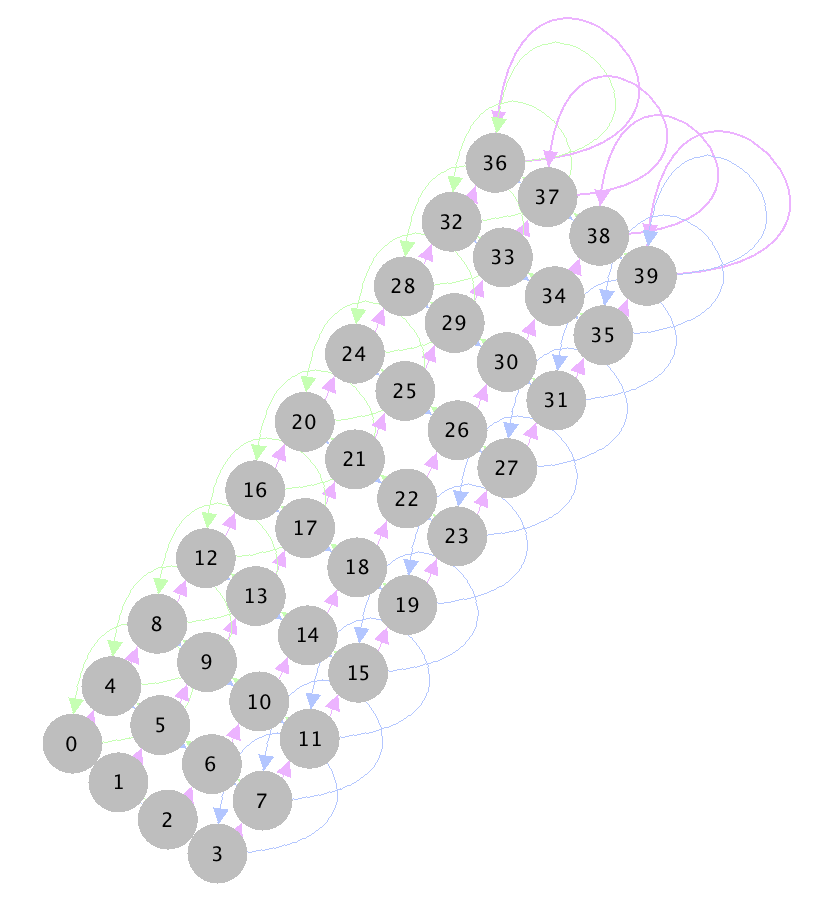
\includegraphics[width=0.48\columnwidth]{figures/ground_upworld.png}}
\subfigure[Abstract UpWorld]{
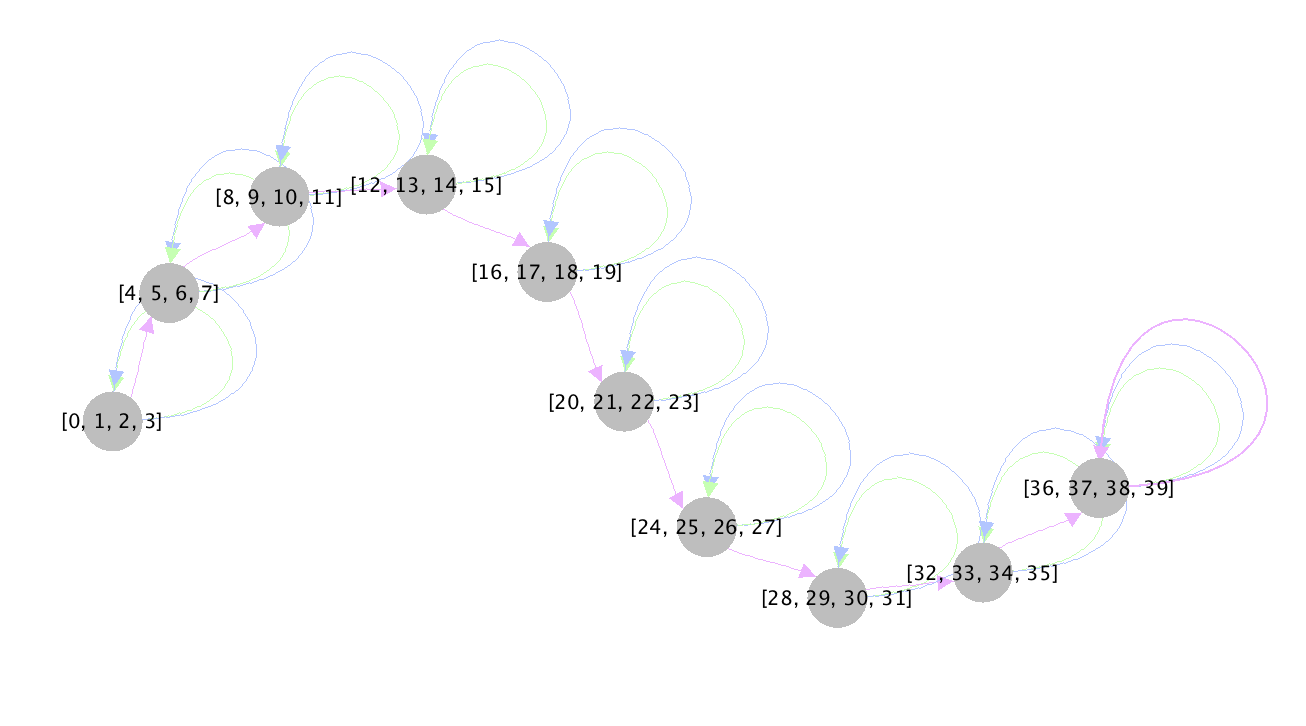
\includegraphics[width=0.48\columnwidth]{figures/abs_upworld.png}}
\label{fig:eps-states}
\caption{Comparison of Original UpWorld MDP and Abstract MDP, under $\epQ$, with $\epsilon=0.5$}
\end{figure} 

% Insert visual and/or stats on number of states and performance of VI solving the abstract MDP and evaluating the resulting policy on the original MDP


% Subsection: NChain.
\subsection{NChain}



% Insert visual and/or stats on number of states and performance of VI solving the abstract MDP and evaluating the resulting policy on the original MDP

\begin{figure}
\subfigure[Ground NChain]{
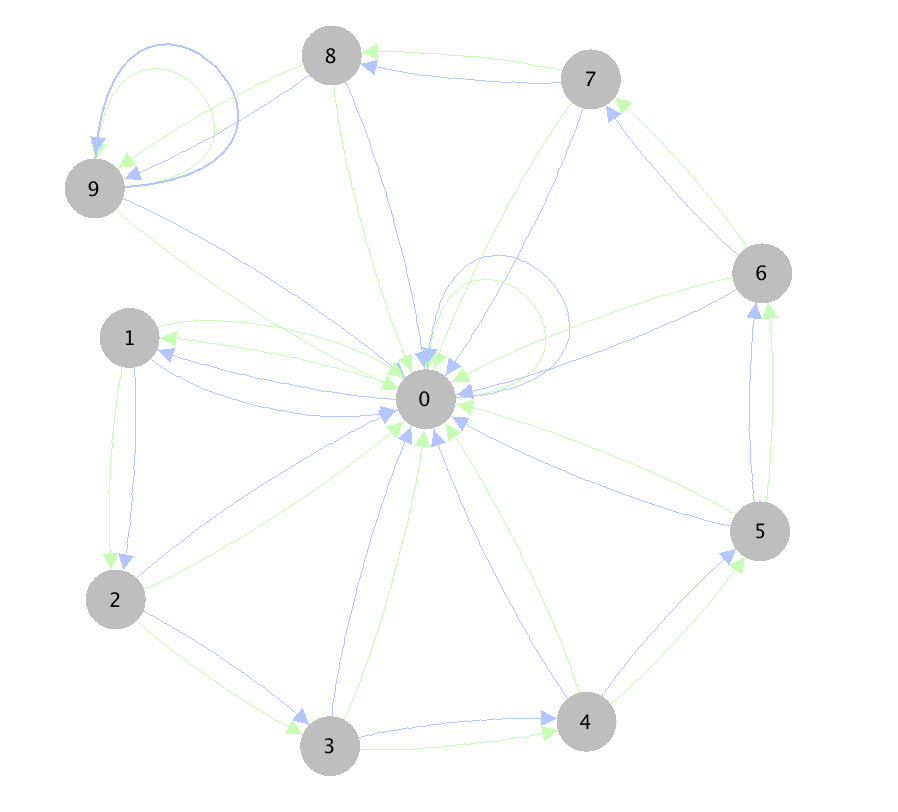
\includegraphics[width=0.48\columnwidth]{figures/ground_nchain.png}}
\subfigure[Abstract NChain]{
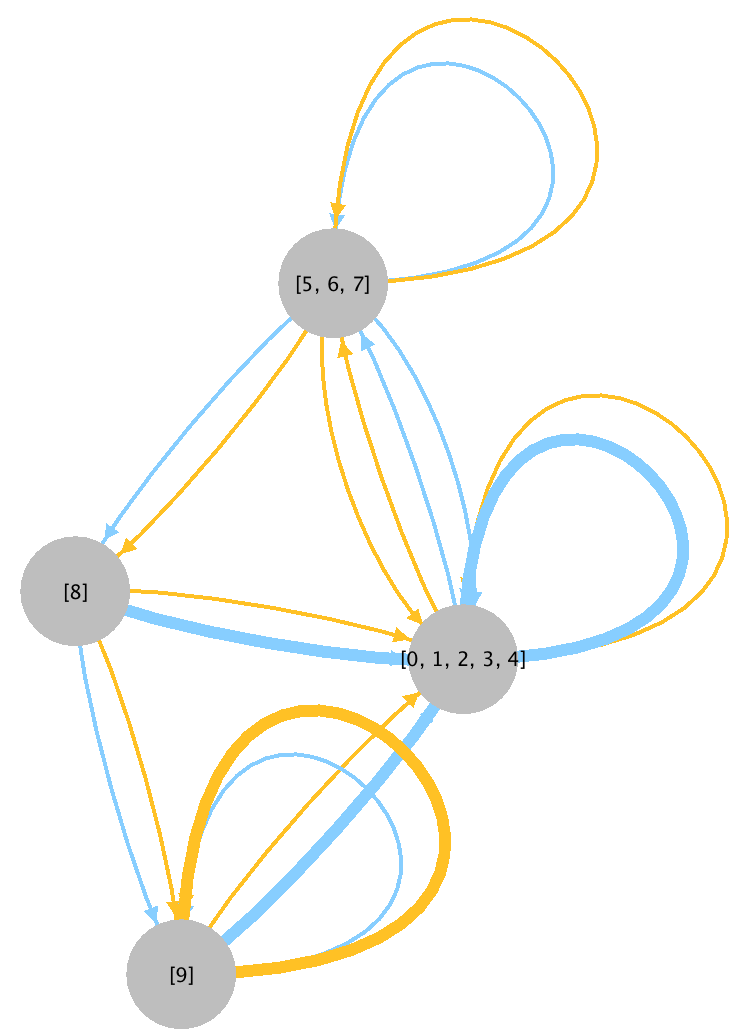
\includegraphics[width=0.48\columnwidth]{figures/abs_nchain.png}}
\label{fig:eps-states}
\caption{Comparison of Original NChain MDP and Abstract MDP, under $\epQ$, with $\epsilon=0.5$}
\end{figure} 

% Subsection: Minefield.
\subsection{Minefield}

Minefield is identical to UpWorld, except the transitions and rewards are perturbed slightly. In particular, there is some slip probability associated with movement; when the agent moves left or right, it has probability $x$ of moving up, when the agent moves up, it has probability $\frac{x}{2}$ of moving left, and probability $\frac{x}{2}$ of moving right. The reward function is nearly identical to UpWorld: transitions to the top row in the grid receive $1.0$ reward, all other transitions receive $0.2$ reward, except for a random set of $\kappa$ states that receive $0$ reward (these are the mine states, that receive $\textsc{RMin}$). During experimentation, we set $N=10, M=4, \epsilon=1.1, \kappa = 5, x = 0.01$.

\begin{figure}
\subfigure[Ground Minefield]{
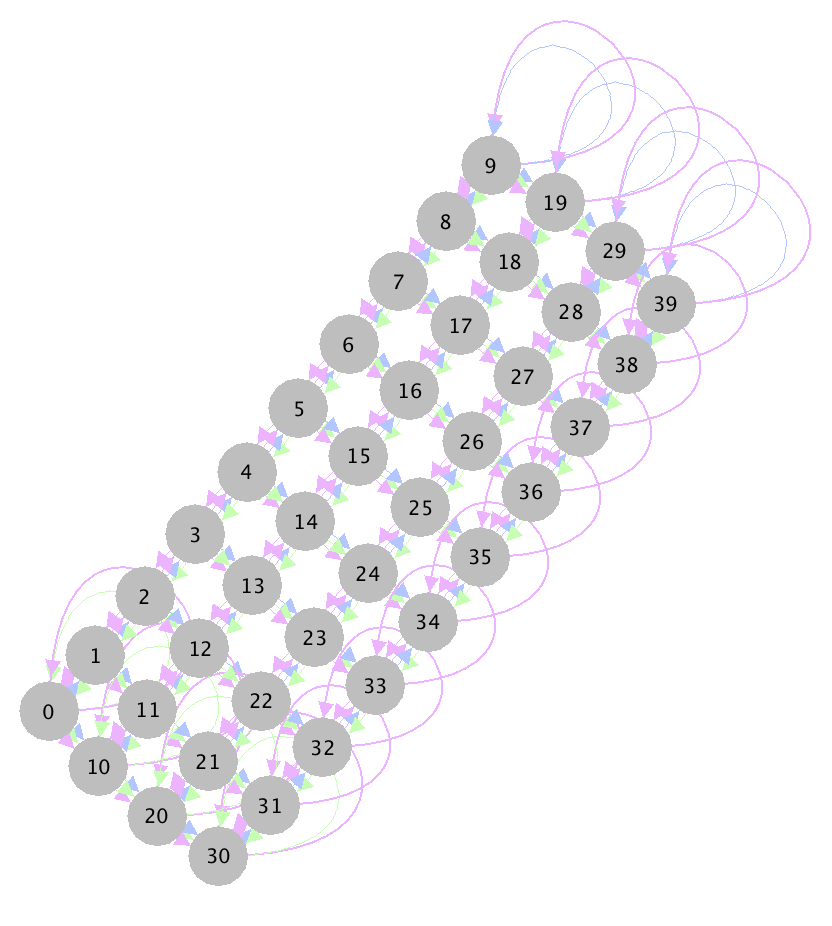
\includegraphics[width=0.48\columnwidth]{figures/ground_minefield.png}}
\subfigure[Abstract Minefield]{
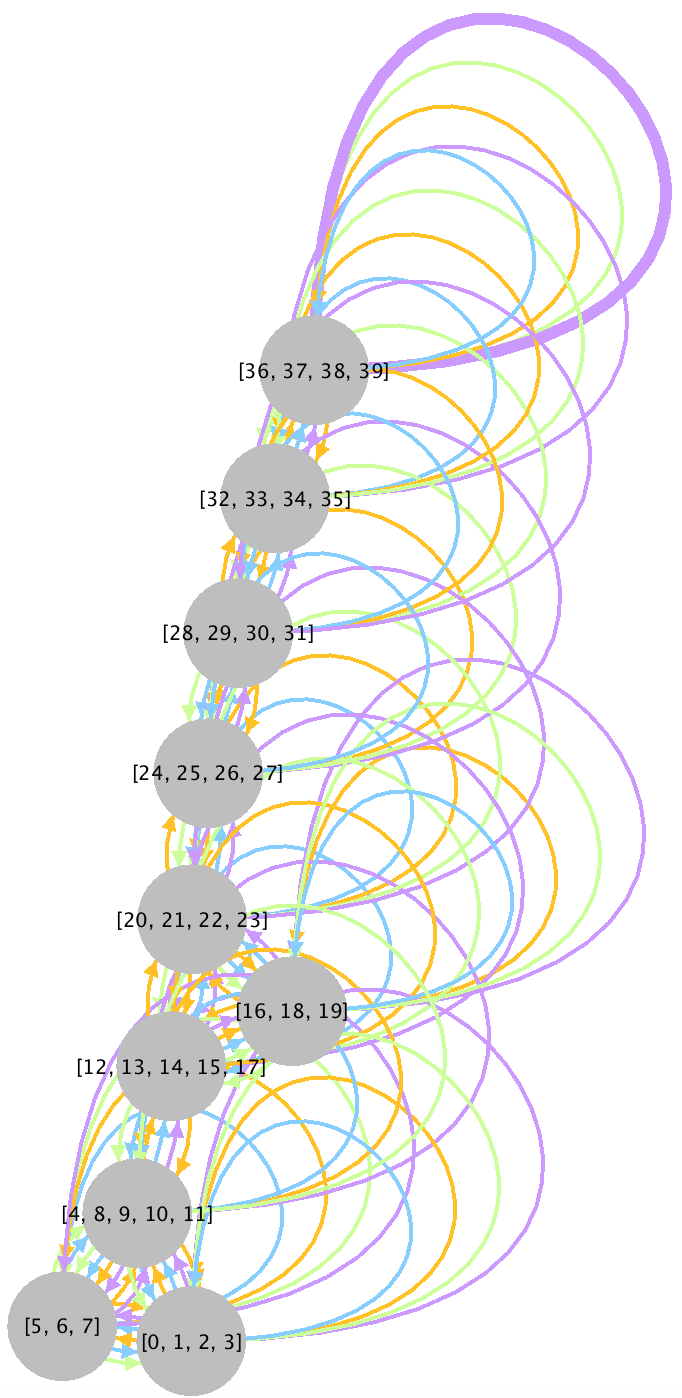
\includegraphics[width=0.48\columnwidth]{figures/abs_minefield.png}}
\label{fig:eps-states}
\caption{Comparison of Original Minefield MDP and Abstract MDP, under $\epQ$, with $\epsilon=1.1$}
\end{figure} 

% Subsection: Trench.
\subsection{Trench}

To demonstrate the effects of approximate abstraction on goal-based tasks, we investigate the Trench problem, introduced by \dnote{Cite dabe}.

% Insert visual and/or stats on number of states and performance of VI solving the abstract MDP and evaluating the resulting policy on the original MDP


% Figure: The Trench Problem
\begin{figure}[h]
\centering
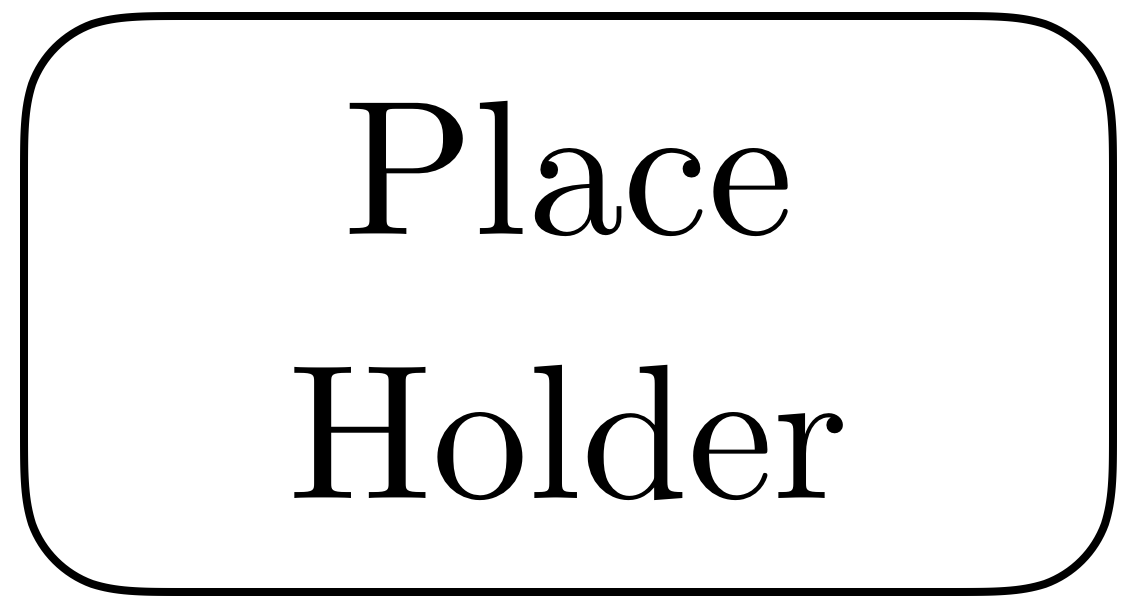
\includegraphics[width=0.42\columnwidth]{figures/placeholder.png}
\caption{The Trench Problem}
\label{fig:trench}
\end{figure}

% Subsection: Minefield.
\subsection{Minefield}


% --- SECTION: Approximate Abstraction on Example Domains ---
\section{Approximate Abstraction on Example Domains}

% Figure: Epsilon vs. #States for all three sample domains.
\begin{figure}
\subfigure[UpWorld]{
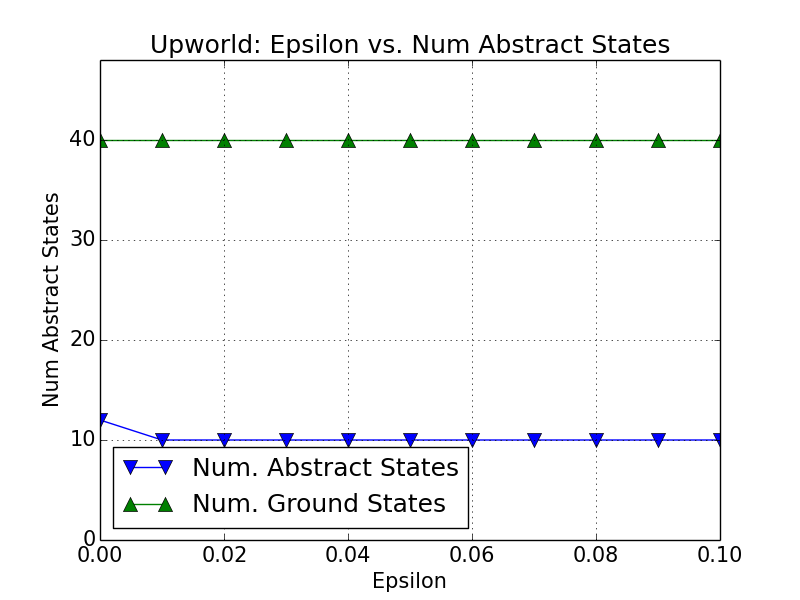
\includegraphics[width=0.28\columnwidth]{figures/upworld_epsilon_vs_num_abstract_states.png}}
\subfigure[NChain]{
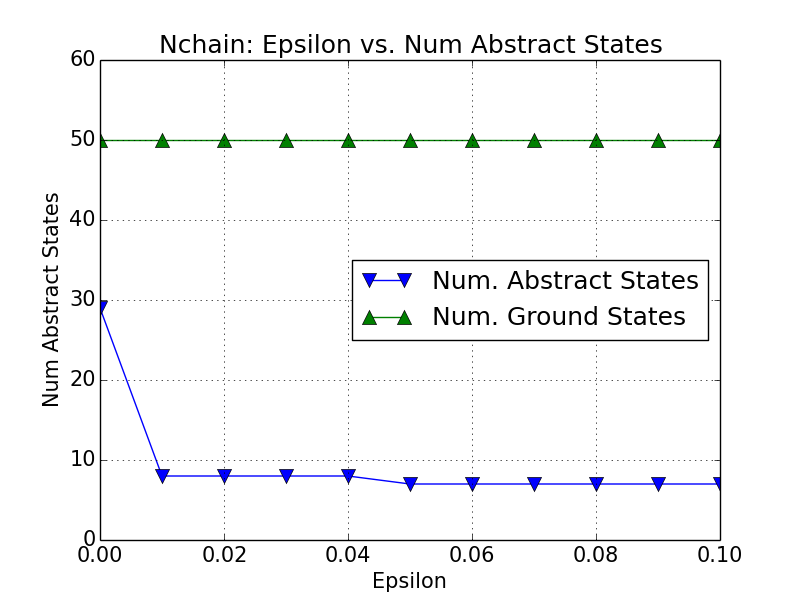
\includegraphics[width=0.28\columnwidth]{figures/nchain_epsilon_vs_num_abstract_states.png}}
\subfigure[Minefield]{
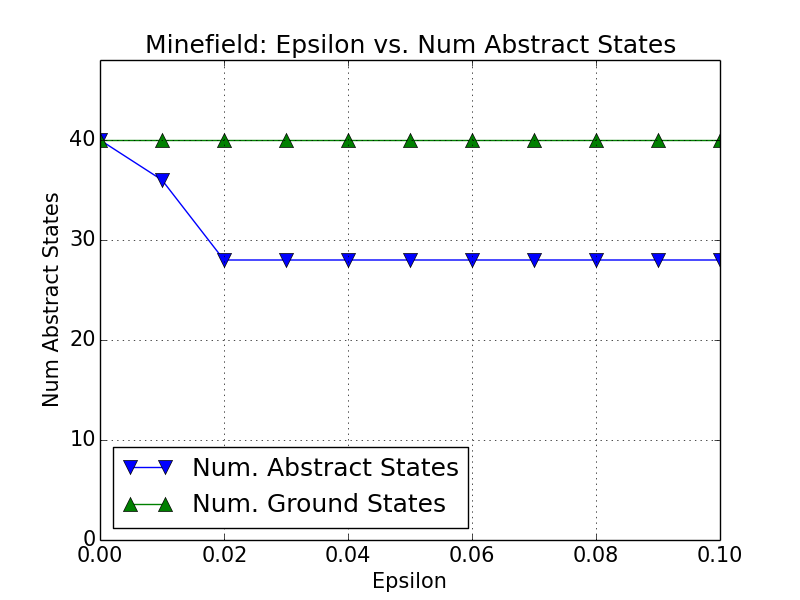
\includegraphics[width=0.28\columnwidth]{figures/minefield_epsilon_vs_num_abstract_states.png}}
\subfigure[Trench]{
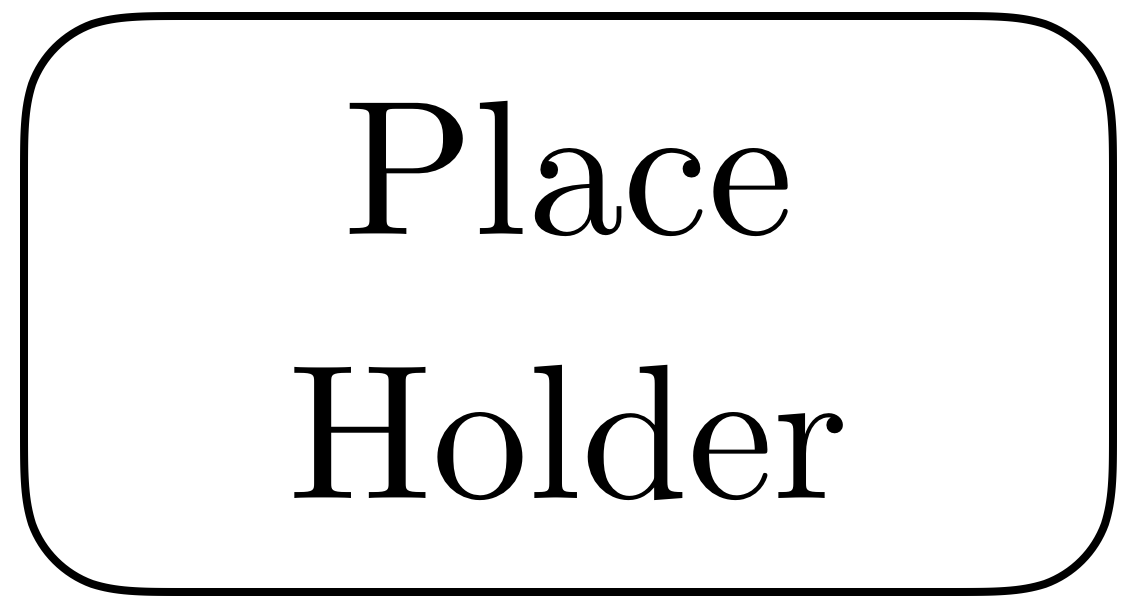
\includegraphics[width=0.28\columnwidth]{figures/placeholder.png}}
\label{fig:eps-states}
\caption{$\epsilon$ vs. Num States}
\end{figure} 

% Figure: Epsilon vs. Error in Abstract Value Function
\begin{figure}
\subfigure[UpWorld]{
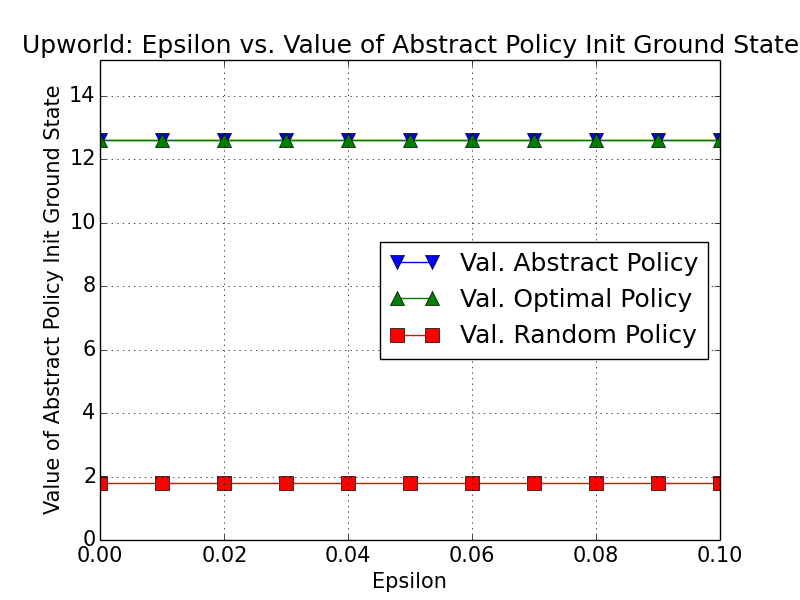
\includegraphics[width=0.28\columnwidth]{figures/upworld_epsilon_vs_value_of_abstract_policy_init_ground_state.png}}
\subfigure[NChain]{
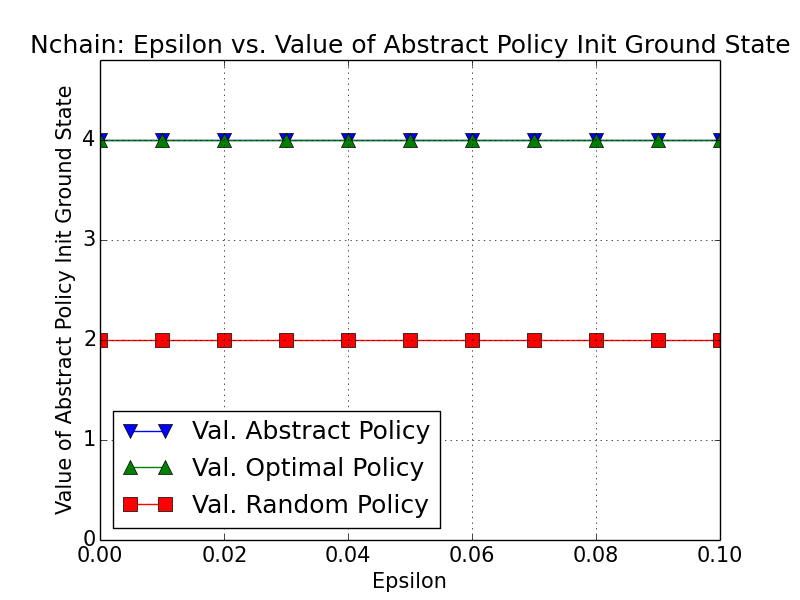
\includegraphics[width=0.28\columnwidth]{figures/nchain_epsilon_vs_value_of_abstract_policy_init_ground_state.png}}
\subfigure[Minefield]{
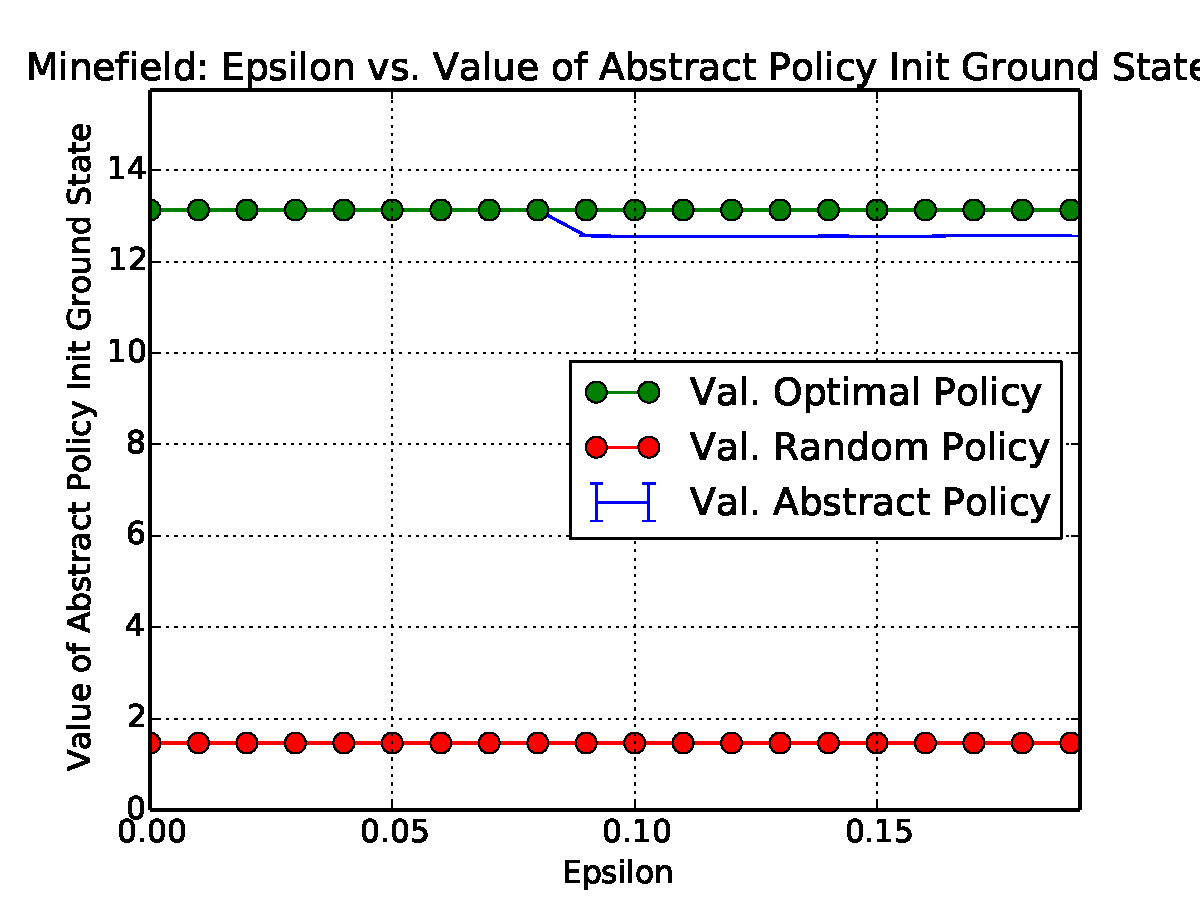
\includegraphics[width=0.28\columnwidth]{figures/minefield_epsilon_vs_value_of_abstract_policy_init_ground_state}}
\label{fig:eps-states}
\caption{$\epsilon$ vs. the Value under the Abstract Policy in the Initial Ground State}
\end{figure} 



% Subsection: Abstract Domain Visualizations
\subsection{Abstract Domain Visualizations}

% Figure: UpWorld MDP visuals
\begin{figure}[h]
\centering
\subfigure[UpWorld]{
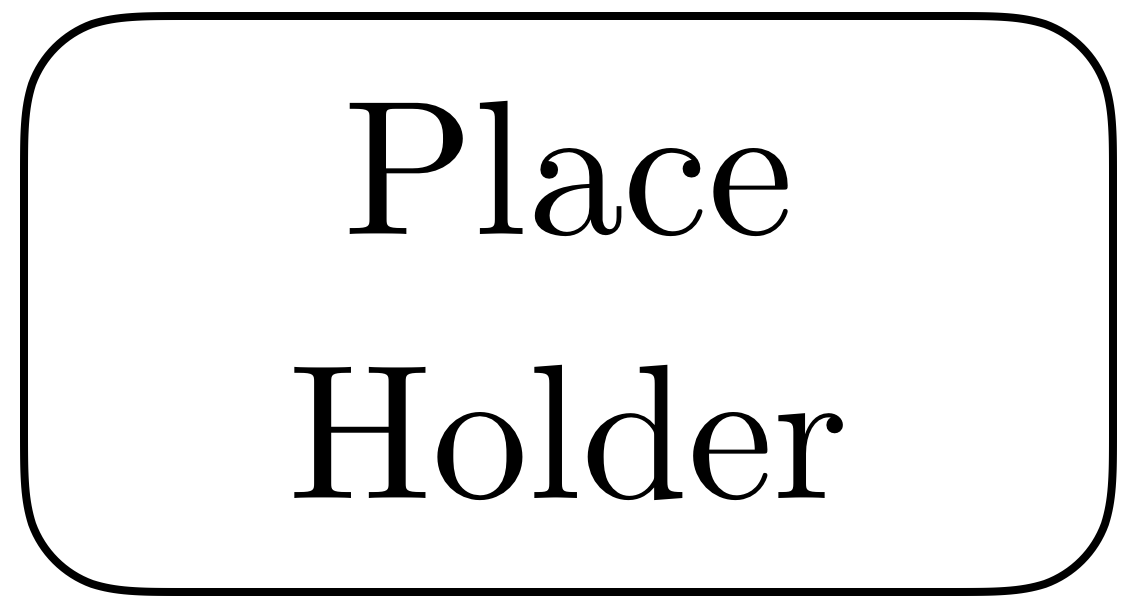
\includegraphics[width=0.46\columnwidth]{figures/placeholder.png}}
\hspace{3mm}
\subfigure[Abstracted UpWorld]{
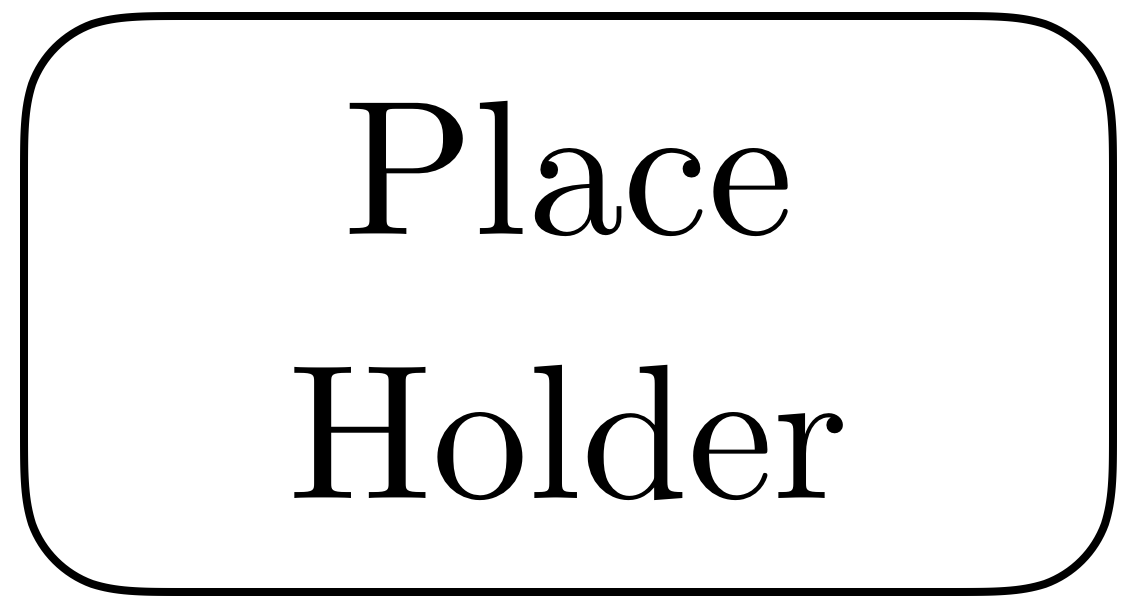
\includegraphics[width=0.46\columnwidth]{figures/placeholder.png}}
\caption{Visualization of Original UpWorld vs. Abstracted UpWorld}
\end{figure}

% Figure: NChain MDP visuals
\begin{figure}[h]
\centering
\subfigure[NChain]{
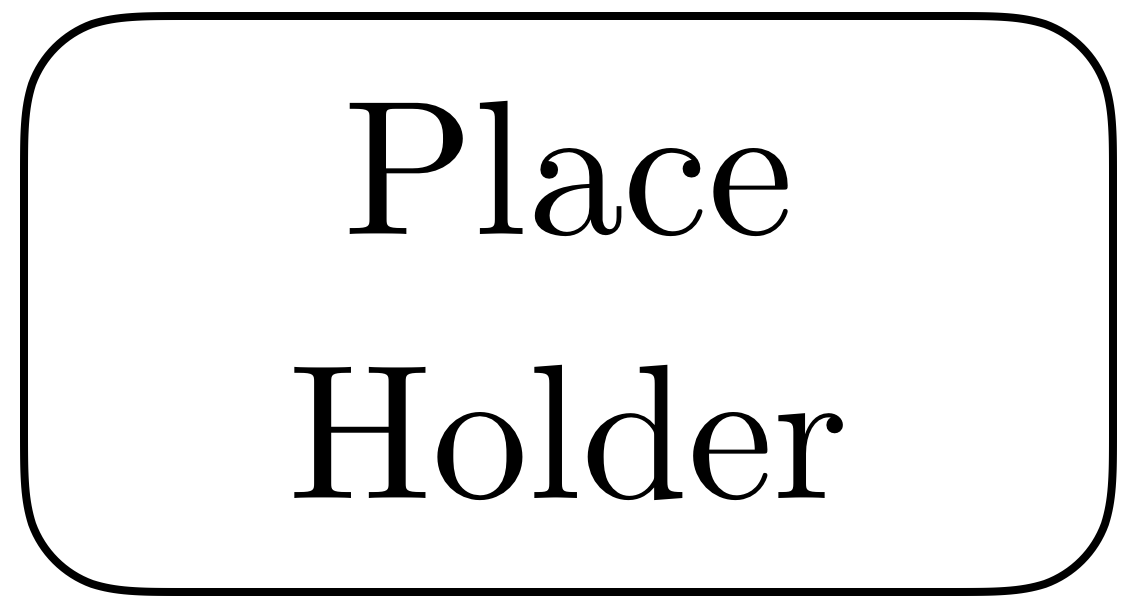
\includegraphics[width=0.46\columnwidth]{figures/placeholder.png}}
\hspace{3mm}
\subfigure[Abstracted NChain ]{
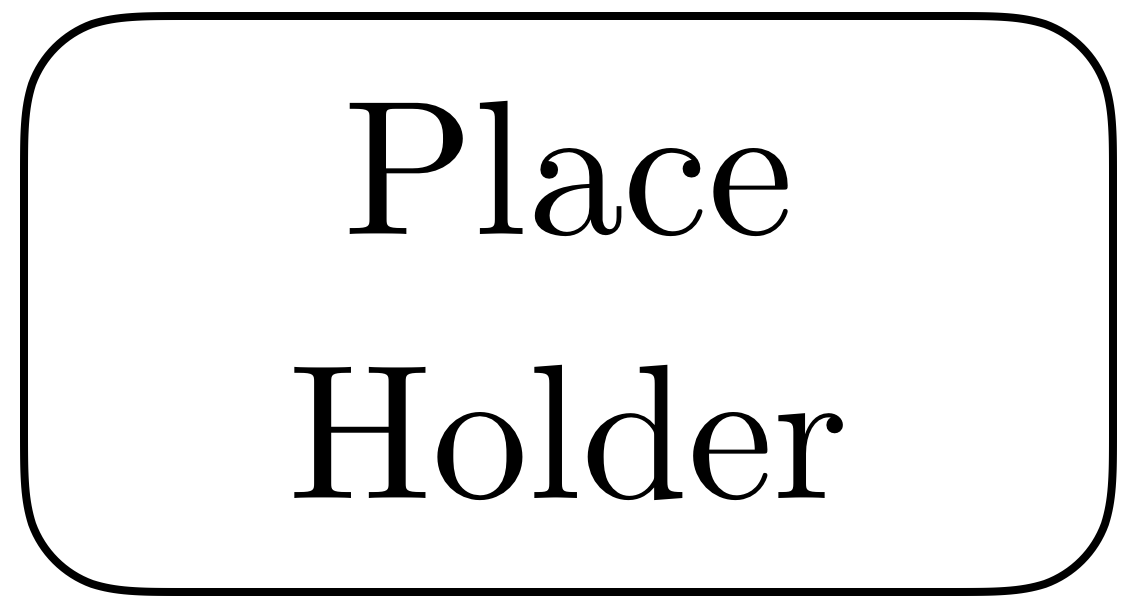
\includegraphics[width=0.46\columnwidth]{figures/placeholder.png}}
\caption{Visualization of Original NChain vs. Abstracted NChain}
\end{figure}






% --- SECTION: Conclusion ---
\section{Conclusion}

% Summary

% Future Work
\begin{enumerate}
\item Learning Phi
\begin{itemize}
\item Exploration vs. Exploitation problem is different while trying to learn Phi
\end{itemize}
\item Compressibility
\begin{itemize}
\item Relationship between approximate abstract and compressibility
\end{itemize}
\item POMDP and abstraction
\end{enumerate}





% --- BIBLIOGRAPHY ---
\bibliographystyle{icml2016/icml2016}
\bibliography{state_abs}

\end{document}
